\section{Интегрируемые ФНП}

\subsection{Измеримые множества в $\RN$}
Для $a_i \in \mathbb{R}, i = \overline{1,n}$ и $b_i \in \mathbb{R}, \text{где } a_i \leqslant b_i, i = \overline{1,n}$ \important{прямоугольным параллелепипедом} в $\RN$ будем называть множество T $\subset \RN$ точек: $M(x) = M(x_1, x_2, \ldots, x_n) \in \RN$ таких, что $a_i \leqslant \forall x_i \leqslant b_i, i = \overline{1,n}$.

Для таких параллелепипедов T $\in \RN$ за \important{меру} mes T примем число:
\begin{equation}
	\label{611}
	\mes \text{T} = (b_1 - a_1) \cdot (b_2 - a_2) \cdot \ldots \cdot (b_n - a_n).
\end{equation}
\textbf{Примеры: } \\
\begin{enumerate}
  \item $n = 1 \Rightarrow \text{T} = \{ x \in \mathbb{R} | a \leqslant x \leqslant b  \}$ - отрезок $[a,b] \in \mathbb{R}, \mes \text{T} = b-a$ - длина данного отрезка.
	\begin{center}
		\begin{tikzpicture}
			\coordinate (left) at (-0.3 * \paperwidth, 0.0);
			\coordinate (right) at (0.3 * \paperwidth, 0.0);
			\coordinate (center) at (0, 0);
			\coordinate (delta) at(4.0, 0);
			\coordinate (delta2) at(3.0, 0);
			\coordinate (delta3) at(-3.0, 0);
			\coordinate (letterdeltabottom) at(0, -0.5);
			\coordinate (letterdeltatop) at(0.0, 0.5);
			\draw (center) ++ (0, 0.5) node {$\text{T}$};
			\draw[->] (center -| left) -- (center -| right);
			\foreach \x in {-2.75, -2.5, ..., 3.0}
			\draw[xshift=\x cm] (0.0, 0.0) -- (-0.1, 0.3);
			\fill[black] (-3.0, 0) circle(0.1);
			\draw (right) node[anchor=north] {$x$};
			% \fill[white] (-3.0, 0) circle(0.07);
			% \fill[black] (center) ++ (delta) circle(0.12);
			% \fill[black] (center) ++ (center) circle(0.1);
			\fill[black] (center) ++ (delta2) circle(0.1);
			% \fill[white] (center) ++ (delta2) circle(0.07);
			%	\draw (0, 0.4) ++ (letterdeltatop) node {$\boxed{\overline{B_r}(x_0)}$};
			%	\draw (center) ++ (letterdeltabottom) node {$x_0$};
			\draw (center) ++ (delta2) ++ (letterdeltabottom) node {$b$};
			\draw (center) ++ (delta3) ++ (letterdeltabottom) node {$a$};
			\ %draw (3.35, 0.15) ++ (delta2) ++ (letterdeltabottom) node {$x$};
			% \draw[fill=black] (-3.0, 0.07) -- (-3.0, 0.51);
			%	\draw[fill=black] (-3.0, 0.51) -- (-2.7, 0.51);
			% \draw[fill=black] (-3.0, -0.07) -- (-3.0, -0.31);
			% \draw[fill=black] (-3.0, -0.31) -- (-2.7, -0.31);
			% \draw[fill=black] (3.0, 0.07) -- (3.0, 0.51);
			% \draw[fill=black] (3.0, 0.51) -- (2.7, 0.51);
			% \draw[fill=black] (3.0, -0.07) -- (3.0, -0.31);
			% \draw[fill=black] (3.0, -0.31) -- (2.7, -0.31);
		\end{tikzpicture}
	\end{center}
  \item $n = 2 \Rightarrow \text{T} = \{ (x,y) \in \mathbb{R}^2 | a_1 \leqslant x \leqslant b_1, a_2 \leqslant y \leqslant b_2  \}$ - прямоугольник T = $[a_1,b_1] \times [a_2,b_2]$ \\
	$\mes \text{T} = (b_1-a_1)(b_2-a_2)$ - площадь данного прямоугольника.
	\begin{center}
		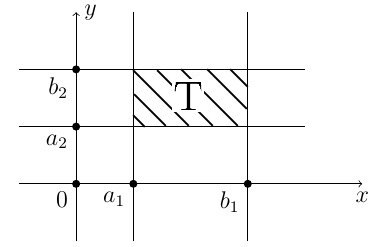
\includegraphics[scale=0.7]{img/633.jpg}
	\end{center}
  \item $n = 3 \Rightarrow \text{T} = \{ (x,y,z) \in \mathbb{R}^3 | a_1 \leqslant x \leqslant b_1, a_2 \leqslant y \leqslant b_2, a_3 \leqslant z \leqslant b_3  \}$ - прямоугольный параллелепипед T = $[a_1,b_1] \times [a_2,b_2] \times [a_3,b_3]$ \\
	$\mes \text{T} = (b_1-a_1)(b_2-a_2)(b_3-a_3)$ - объём данного прямоугольного параллелепипеда.
	\begin{center}
		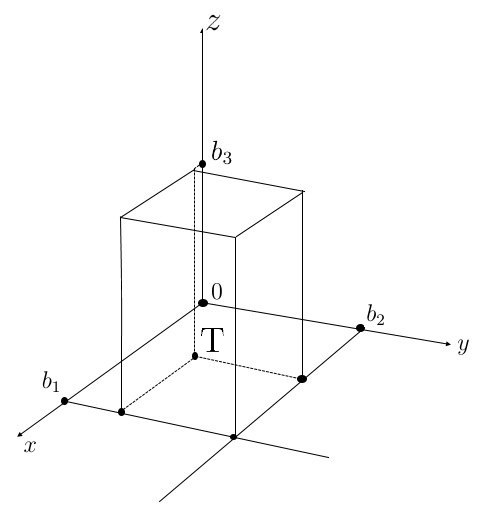
\includegraphics[scale=0.6]{img/634.jpg}
	\end{center}
\end{enumerate}

\important{Многогранником} $H \subset \RN$ будем называть произвольное конечное объединение параллелепипедов в $\RN$.

Если этот многогранник разбит на конечное число  составляющих параллелепипедов $\text{T}_k, k = \linebreak = \overline{1,m}$, у каждого из которых общими могут быть лишь граничные точки, т.е. $H = \bigcup\limits_{k=1}^m \text{П}_k$, то в этом случае полагают:
\begin{equation}
	\label{612}
	\mes H = \sum\limits_{k=1}^{m} \mes \text{T}_k.
\end{equation}
В дальнейшем считаем, что для пустого множества $\mes \emptyset = 0$.

Можно показать, что \eqref{612} не зависит от способа разбиения H на составляющие его параллелепипеды.

Для произвольного $D \subset \RN$ многогранник H считается \important{вписанным} в $D$, если $H \subset D$, и многогранник S считается  \important{описанным} около $D$, если $D \subset S$.

Величины
\begin{equation}
	\label{613}
	\begin{cases}
		m_* = \underset{\forall H \subset D}{\sup} \{ \mes H \}, \\
		m^* = \underset{\forall S \supset D}{\inf} \{ \mes S \},
	\end{cases}
\end{equation}
называются соответственно \important{нижней мерой} для D и \important{верхней мерой} для D.

По теореме о гранях, эти меры существуют (конечные или бесконечные).

В случае, когда $ m^* = m_{*} \in \mathbb{R} $,
множество $ D $ называется  \important{измеримым по Жордану} в пространстве $\RN$ и за его меру принимается $\mes D = m^* = m_{*}$.

Необходимым условием существования конечной меры (измеримости) по Жордану является ограниченность рассматриваемого множества $D \subset \RN$. В дальнейшем множество $D_0 \subset \RN$ будем называть \important{множеством меры нуль}, если для $\forall\; \varepsilon > 0 \;\;\; \exists\; H_\varepsilon \subset D_0$ и $\exists S_\varepsilon \supset D_0$, такие, что

\begin{equation}
	\label{614}
	\mes S_\varepsilon - \mes H_\varepsilon \leqslant \varepsilon,
\end{equation}
где $S_\varepsilon, H_\varepsilon$ - соответствующие многогранники в $\RN$.
\newpage
Для множеств меры нуль имеем следующие \important{свойства}:
\begin{enumerate}
  \item Пустое множество, одноточечное множество и множество, состоящее из конечного числа точек в $\RN$, является множеством меры нуль.
  \item Объединение конечного или счётного числа множеств меры нуль в $\RN$ будем множеством меры нуль.
  \item Любое подмножество множества меры нуль имеет нулевую меру.
\end{enumerate}
Критерием измеримости множества $D \subset \RN$ является его ограниченность и условие, что мера границы равна нулю ($ \mes \partial D = 0 $).

В общем случае для $\forall D_1, D_2 \subset \RN$ (любых измеримых) имеем:
\begin{equation}
	\label{615}
	mes (D_1 \cup D_2) = \mes D_1 + \mes D_2 - \mes(D_1 \cap D_2).
\end{equation}
Если в \eqref{615} мера пересечения $\mes(D_1 \cap D_2) = 0$, то имеем:
\begin{equation*}
    \mes (D_1 \cup D_2) = \mes D_1 + \mes D_2,
\end{equation*}
что выражает свойство конечной аддитивности меры Жордана в $\RN$.

Аналогично, если мера $\mes(D_i \cap D_j) = 0, \forall i \ne j, i = \overline{1,m}, j = \overline{1,m}$, то методом математической индукции (ММИ) доказывается, что
\begin{equation}
	\label{616}
	\mes \left(\bigcup_{k=1}^m D_k \right) = \sum_{k=1}^{m} \mes D_k.
\end{equation}

Равенство \eqref{616} заведомо выполняется для измеримых множеств в $D_k \in \RN, k = \overline{1,m}$ в случае, когда у них общими могут быть лишь граничные точки.

\subsection{Интегральные суммы и интеграл ФНП}

Для измеримого множества $D \subset \RN$ рассмотрим произвольное разбиение ${\forall P = \set{P_k}}$, ${k = \overline{1, m}}$, где $\forall P_k \subset D$ измеримы в $D$, и они имеют между собой
общими лишь может быть только граничные точки. В этом случае:
\begin{equation*}
	D = \bigcup\limits_{k = 1}^m P_k\; \text{ и } \mes(P_i \cap P_j) = 0, i \neq j; i, j = \overline{1, m}.
\end{equation*}

Выбирая произвольным образом отмеченное множество точек $Q = \set{M_k}, \forall M_k \in P_k, $
$k = \overline{1, m}$,
для ФНП $f(x)$, определённой для $\forall x \in D \subset \RN$ рассмотрим интегральную сумму:
\begin{equation}
	\label{eq:6.2-integral-sum}
	\sigma = \sigma(f, \{P; Q\}) = \sum\limits_{k = 1}^mf(M_k)\Delta{P_k},
\end{equation}
где $\Delta{P_k} = \mes P_k, k = \overline{1, m}$.

В дальнейшем величину $r_k = \max d(A; B)$, где $ \forall A, B \in P_k$, будем называть \important{диаметром}
множества $P_k \subset D$. Геометрически $r_k$ представляет собой диаметр $n$-мерного шара
наименьшего размера, содержащего $P_k$.

% Для краткости введём обозначение $r_k = \diam P_k, k = \overline{1, m}$.
Величину
${r = \max\set{r_k}}$, ${1 \leqslant k \leqslant m}$, будем называть \important{диаметром} используемого разбиения и
обозначать $r = \diam P$.

Функция $f(x)$, определённая для $x = (x_1, \ldots, x_n) \in D$, где $D \subset \RN$- измеримое
множество, считается интегрируемой на $D$, если
\begin{equation}
    \label{eq:6.2-integrity-definition}
	\exists I \subset \RN, \text{ что для }\forall \varepsilon > 0, \exists \delta > 0, \forall \set{P; Q},
	r = \diam P \leqslant \delta \Rightarrow \abs{I  - \delta}
	\overset{\eqref{eq:6.2-integral-sum}}{\leqslant} \varepsilon.
\end{equation}

Число $ I \in \mathbb{R} $ в \eqref{eq:6.2-integrity-definition}
будем называть значением $n$-кратного интеграла.
\begin{equation*}
	I = \underset{D}{\iint\ldots\int} f(x_1, \ldots, x_n) d x_1 \ldots dx_n = \int\limits_{D}f(x)dx
\end{equation*}

В дальнейшем будем также писать $I \overset{\eqref{eq:6.2-integral-sum}-
  \eqref{eq:6.2-integrity-definition}}{=}{\lim\limits_{r \to 0} \sigma}$.

При $n = 2$ для $ D \subset \mathbb{R}^2 $ интеграл \eqref{eq:6.2-integrity-definition} будем называть двойным (2И) и
обозначать в прямоугольной декартовой системе координат $Oxy$:
\begin{equation*}
\label{eq:6.2-double-integral}
I = \iint\limits_{D }f(x, y)dxdy,
\end{equation*}
а при $n = 3$ для $ D \subset \mathbb{R}^3 $ интеграл \eqref{eq:6.2-integrity-definition} будем называть тройным (3И) и обозначать в прямоугольной декартовой системе координат $Oxyz$:
\begin{equation*}
I = \iiint\limits_{D }f(x, y, z)dxdydz.
\end{equation*}

\begin{example}
	Пусть $f(x) \equiv 1, \forall x \in D \subset \RN$, где $D$ - измеримое множество. В этом
	случае
	\begin{equation*}
		\sigma 	\overset{\eqref{eq:6.2-integral-sum}}{=} \sum\limits_{k = 1}^m\Delta{P_k} =
		\sum_{k = 1}^m \mes P_k
	\end{equation*}
	поэтому в данном случае:
	\begin{equation}
		\label{eq:6.2-integral-example1}
        I = \lim\limits_{r \to 0}\sigma = \lim\limits_{r \to 0}(\mes D) = \mes D, \text{ т.е. }
		\int\limits_D dx = \mes D.
	\end{equation}
\end{example}

Равенство \eqref{eq:6.2-integral-example1} выражает простейший геометрический смысл $n$-кратного интеграла.
\begin{itemize}
  \item В случае $n = 1$ \eqref{eq:6.2-integral-example1} соответствует длине используемого отрезка
	интегрирования \\${D = \interval[{a; b}] \subset \R{}}$ ${(\mes D = b - a)}$.
  \item В случае $n = 2$ \eqref{eq:6.2-integral-example1} выражает площадь из $D \subset \R{2}$ в прямоугольной декартовой системе координат $Oxy$:
	\begin{equation*}
		\mes D = \iint\limits_{D \subset \R{2}}dxdy = \text{Площадь } D.
	\end{equation*}
  \item В случае $n = 3$ для измеримого $D \subset \R{3}$ получаем объём в прямоугольной декартовой системе координат $Oxyz$:
	\begin{equation*}
		\mes D = \iiint\limits_{D \subset \R{3}}dxdydz = \text{Объём } D.
	\end{equation*}
\end{itemize}

Как и для однократного интеграла ($n = 1$), множество интегрируемых на $D \subset \RN$ функций будем обозначать
$\mathbb{R}(D)$. Имеем следующие основные свойства $n$-кратных интегралов:
\begin{enumerate}
  \item \important{Линейность}\\
	Если $f, g \in \mathbb{R}(D)$для измеримого $D \subset \RN$, то
	\begin{equation*}
		\begin{split}
			&\forall \lambda, \mu \in \mathbb{R} \Rightarrow (\lambda f + \mu g) \in \mathbb{R}(D),\text{ причём} \\
			&\int\limits_D (\lambda f(x) + \mu g(x))dx = \lambda \int\limits_D f(x)dx +
			\mu \int\limits_D g(x)dx.
		\end{split}
	\end{equation*}
  \item \important{Аддитивность}\\
	Если $f \subset \mathbb{R}(D), D = D_1 \bigcup D_2$, где $D_1$, $D_2$ - измеримые множества в $\RN$,
	общими у которых могут быть лишь только граничные точки (${ \mes(D_1 \cap D_2) = 0 }$), то:
	\begin{equation*}
		\int\limits_{D}fdx = \int\limits_{D_1}fdx + \int\limits_{D_2}fdx.
	\end{equation*}
  \item \important{Неотрицательность}\\
	Пусть $f \in \mathbb{R}(D)$ и
    $ \forall x \in D \subset \RN \Rightarrow f(x) \geqslant 0 $, где
	$D$ - измеримое множество в $\RN$. Тогда:
	\begin{equation*}
		\int\limits_Df(x)dx \geqslant 0.
	\end{equation*}
  \item \important{Монотонность}\\
	Если $f, g \in \mathbb{R}(D)$ и $\forall x \in D \subset \RN \Rightarrow f(x) \leqslant g(x)$,
	где $D$ - измеримое множество в $\RN$, то:
	\begin{equation*}
		\int\limits_Df(x)dx \leqslant \int\limits_Dg(x)dx.
	\end{equation*}
  \item \important{Основная оценка}\\
	Пусть $\forall x \in D \subset \RN \Rightarrow m_0 \leqslant f(x) \leqslant M_0$, где
	$m_0, M_0 \in \mathbb{R}$, а $D$ - измеримое множество в $\RN$. Тогда:
	\begin{equation*}
		m_0 \mes D \leqslant \int\limits_D f(x) dx \leqslant M_0 \mes D.
	\end{equation*}
\end{enumerate}

Обоснование всех этих свойств проводится по той же схеме, что и для однократного интеграла.

Аналогично Ф1П обосновываются критерий Гейне и критерий Коши интегрируемости ФНП,
а также $C$-лемма для критерия Коши интегрируемости ФНП. На основании этого, так же, как и для
однократных интегралов, доказывается
\begin{theorem}[об интегрируемости непрерывных ФНП]
    $  $

	Если $f \in C(D)$, т.е. непрерывна на измеримом компакте $D \subset \RN$, то $f \in \mathbb{R}(D)$,
	т.е. интегрируема на $D$.
\end{theorem}

\newpage
\begin{consequence}[теорема о среднем для ФНП]

	Пусть $f \in C(D)$, а $g \subset \mathbb{R}(D)$, где $D \subset \RN$ - измеримый компакт. Если
	$\forall x \in D $ функция $g(x)$ сохраняет один и тот же знак, то $\exists x_0 \in D \subset \RN \Rightarrow$
	\begin{equation}
		\label{eq:6.2-intermediate-value}
        % \Rightarrow
		\int\limits_D f(x)g(x)dx =
		f(x_0)\int\limits_Dg(x)dx.
	\end{equation}
	Доказательство по той же схеме, что и для Ф1П.
\end{consequence}

\begin{note}
	Если взять в \eqref{eq:6.2-intermediate-value} $g(x) \equiv 1, \forall x \in D$, то, учитывая
	предыдущий пример, получаем:
	\begin{equation*}
		\text{если } f \in C(D), \text{ то }\exists x_0 \in D \text{ такое, что } \int\limits_Df(x)dx = f(x_0) \mes D,
	\end{equation*}
	что соответствует простейшей теореме о среднем для непрерывной, а значит, интегрируемой, ФНП.
\end{note}

\subsection{Двойной интеграл (2И)}

Рассмотрим функцию $f(x,y), \forall (x,y) \in D \subset \mathbb{R}^2$, где $D$ - измеримое множество в $\mathbb{R}^2$, т.е. плоская квадрируемая фигура. В этом случае имеем 2И:
\begin{equation}
	\label{eq:6.2-11}
	I = \iint\limits_{D} f(x,y)dxdy.
\end{equation}
\begin{theorem}[о вычислении 2И по прямоугольнику для непрерывных Ф2П]
	Пусть $f(x)$ непрерывна на прямоугольнике: П $= [a;b]\times[c;d] = \defineset{(x,y) \in \mathbb{R}^2 }{a \leq x \leq b, c \leq y \leq d}$.

	Тогда для \eqref{eq:6.2-11} следует:
	\begin{equation}
		\label{eq:6.2-12}
		I = \int\limits_{a}^b \left(\int\limits_{c}^d f(x,y)dy\right)dx =  \int\limits_{c}^d \left(\int\limits_{a}^b f(x,y)dx\right)dy.
	\end{equation}
\end{theorem}
\begin{proof}
	Рассмотрим произвольное разбиение: $\widetilde{P} = \{ x_i \}, i = \overline{1,m}$ отрезка $[a;b]: $\\ $a = x_0 < x_1 < \ldots < x_{i-1} < x_i < x_{i+1} < \ldots < x_m = b$ и произвольное разбиение: $\bar{P} = \{y_j\}, j = \overline{1,l}$ отрезка $[c;d]: c = y_0 < y_1 < \ldots < y_{j-1} < y_j < y_{j+1} < \ldots < y_l = d$.

	С помощью вертикальных прямых $x = x_i, i = \overline{1, m}$ и горизонтальных прямых $y = y_j,$ \\$ j = \overline{1, l}$ прямоугольник П $= [a;b]\times[c;d]$ разобьётся на части $ \text{П}_{i,j}= [x_{i-1};x_i]\times[y_{j-1};y_j]$, образующие соответствующее разбиение П = $\bigcup\limits_{i = 1}^m \bigcup\limits_{j = 1}^l \text{П}_{i,j}$ на  составляющие его прямоугольника $\text{П}_{i,j}$, у которых общими могут быть лишь граничные точки.

	\begin{center}
		\begin{tikzpicture}
			\coordinate (left) at (-1.0, 0.0);
			\coordinate (right) at (5.0, 0.0);
			\coordinate (top) at (0.0, 3);
			\coordinate (bottom) at (0.0, -1.0);
			\coordinate (center) at (0.0, 0.0);
			\draw[->] (left) -- (right);
			\draw[->] (bottom) -- (top);
			\draw (right) node[anchor=north] {$x$};
			\draw (top) node[anchor=west] {$y$};
			% \fill [black] (1.5, 1.5) circle (20pt);
			% \fill [white] (1.5, 1.5) circle (19pt);
			% Bottom part of plot
			% \draw[black, dashed] (1.5,1.5) circle (19pt);
			% \draw (1.5,1.5) circle (19pt);
			\draw[fill=black] (-0.5, -0.5) -- (3.0, -0.5);
			\draw[fill=black] (-0.5, -0.5) -- (-0.5, 2);
			\draw[fill=black] (3.0, 2.0) -- (-0.5, 2);
			\draw[fill=black] (3.0, 2.0) -- (3.0, -0.5);

			\draw[fill=black, dashed] (3.0, 1.2) -- (-0.5, 1.2);
			\draw (-0.5, 1.2) node[anchor=north east] {$y_{j-1}$};
			\fill [black] (-0.5, 1.2) circle (2pt);
			\draw (-0.5, 1.5) node[anchor=south east] {$y_{j}$};
			\fill [black] (-0.5, 1.5) circle (2pt);
			\draw[fill=black, dashed] (3.0, 1.5) -- (-0.5, 1.5);

			\draw (0.5, -0.5) node[anchor=north] {$x_{i-1}$};
			\fill [black] (0.5, -0.5) circle (2pt);
			\draw[fill=black, dashed] (0.5, -0.5) -- (0.5, 2);
			\draw (0.8, -0.5) node[anchor=north west] {$x_{i}$};
			\fill [black] (0.8, -0.5) circle (2pt);
			\draw[fill=black, dashed] (0.8, -0.5) -- (0.8, 2);
			\draw (0,-0.5) node[anchor=north east] {$c$};
			\fill [black] (0,-0.5) circle (2pt);
			\draw (0,2) node[anchor=south west] {$d$};
			\fill [black] (0,2) circle (2pt);
			\draw (-0.5,0) node[anchor=north east] {$a$};
			\fill [black] (-0.5,0) circle (2pt);
			\draw (3,0) node[anchor=north west] {$b$};
			\fill [black] (3,0) circle (2pt);
			
			\draw (0.8,2.1) node[anchor=north west] {$\text{П}_{i,j}$};
			\draw[fill=black] (0.8, 1.2) -- (0.5, 1.5);
			\draw[fill=black] (0.8, 1.3) -- (0.6, 1.5);
			\draw[fill=black] (0.8, 1.4) -- (0.7, 1.5);
			\draw[fill=black] (0.7, 1.2) -- (0.5, 1.4);
			\draw[fill=black] (0.6, 1.2) -- (0.5, 1.3);
			% \fill [black] (1.5,1.5) circle (2pt);
			% \fill [black] (1.5,0) circle (2pt);
			% \fill [black] (0, 1.5) circle (2pt);
			% \draw (1.37,1.37) node[anchor=south west] {$\boldsymbol{M_0}$};
			% \draw (1.5,-0.06) node[anchor=north] {$a$};
			% \draw (-0.06, 1.5) node[anchor=east] {$b$};
		\end{tikzpicture}
	\end{center}

	Так как $f \in C(\text{П}) $, то $ f \in C(\text{П}_{i,j}), \forall i = \overline{1,m}, \forall j = \overline{1,l}$.

	Рассмотрим функцию $F_i(y) = \dint\limits_{x_{i-1}}^{x_i} f(x,y)dx, i = \overline{1,m}$.

    Этот интеграл существует, т.к. $\forall \fix y \Rightarrow f(x,y)$ - непрерывна по x. По теореме о среднем для однократных интегралов получаем, что:\\
	$\exists t_{i,j} \in [x_{i-1}; x_i] \Rightarrow F_i(y_j) = \dint\limits_{x_{i-1}}^{x_i} f(x,y_j)dx = f(t_{i,j}, y_j) \Delta x_i$, где $\Delta x_i = x_i - x_{i-1}, i = \overline{1,m}$.

	В соответствии с этим определены точки $M_{i,j} = (t_{i,j}, y_j) \in \text{П}_{i,j}$.

	Таким образом, для прямоугольника П имеем разбиение $P = \{ \text{П}_{i,j} \} $ с множеством отмеченных точек $Q = \{M_{i,j} \}$. Для получаемой специальной интегральной суммы
	\begin{equation}
		\label{eq:6.2-13}
		\sigma = \sigma \left(f; \{P; Q\}\right) = \sum\limits_{i=1}^{m} \sum\limits_{j=1}^{l} f\left(M_{i,j}\right) \Delta \text{П}_{i,j},
	\end{equation}
	где $\Delta \text{П}_{i,j}$ = площадь $\text{П}_{i,j} = (x_i - x_{i-1})(y_j - y_{j-1}) = \Delta x_i \Delta y_j:$
	\begin{equation*}
		\begin{cases}
			\Delta x_i = x_i - x_{i-1}, i = \overline{1,m}, \\
			\Delta y_j = y_j - y_{j-1}, j = \overline{1,l},
		\end{cases}
	\end{equation*}
	имеем $\displaystyle \sigma = \sum\limits_{j=1}^{l} \sum\limits_{i=1}^{m} f(M_{i,j}) \Delta x_i \Delta y_j = \sum\limits_{j=1}^{l} \sum\limits_{i=1}^{m} F_i(y_j) \Delta y_j = \sum\limits_{j=1}^{l} \sum\limits_{i=1}^{m} \left(\nullFrac\dint\limits_{x_{i-1}}^{x_i} f(x,y_j) dx\right) \Delta y_j = \\
	= \begin{sqcases}\sum\limits_{i=1}^{m} \dint\limits_{x_{i-1}}^{x_i} f(x,y) dx = \dint\limits_{x_{1}}^{x_2} + \dint\limits_{x_2}^{x_3} + \ldots + \dint\limits_{x_{n-1}}^{x_n} = \dint\limits_{x_{1}}^{x_n} f(x,y)dx = \dint\limits_{a}^{b} f(x,y)dx   \end{sqcases} = $
	\begin{equation}
		\label{eq:6.3-14}
		= \sum\limits_{j=1}^{l} \left( \dint  \limits_{a}^{b}  f(x, y_j) dx \right) \Delta y_j
		=\sum\limits_{j=1}^{l} F(y_j) \Delta y_j,
	\end{equation}
	где
	\begin{equation}
		\label{eq:6.3-15}
		\begin{cases}
			F(y) = \dint\limits_{a}^{b} f(x,y) dx, \\
			y \in [a; b].
		\end{cases}
	\end{equation}
	Из \eqref{eq:6.3-14} следует, что $\sigma$ является одной из интегральных сумм для \eqref{eq:6.3-15}, вычисляемых на разбиении $\bar{P} = \{y_j\}, j = \overline{1, l}$. Отсюда при $\bar{r} = diam \bar{P} = \underset{1 \leqslant j \leqslant l}{max}\{\Delta y_j\} \to 0$, в силу непрерывности используемых функций следует:
	${\exists \dint\limits_c^d F(y)dy = \lim\limits_{\bar{r} \to 0} \sum\limits_{j=1}^{l} F(y_j) \Delta y_j = [\eqref{eq:6.3-14}] = \lim\limits_{\bar{r} \to 0} \sigma = I}$.

	В силу того, что из непрерывности функций следует их интегрируемость, а значит, возможность использования для вычисления $I$ не общих интегральных сумм, а специальных, получаем, что:
    % \begin{equation*}
    $
	I =  \dint\limits_{c}^{d} F(y) dy \overset{\eqref{eq:6.3-15}}{=} \dint\limits_c^d \left(\dint\limits_a^b f(x,y)dx \right) dy.
    $
    % \end{equation*}

	Аналогично доказывается и второе равенство \eqref{eq:6.2-12}.
\end{proof}

\newpage

\begin{notes}
  \item На практике формулы \eqref{eq:6.2-12} записываются в виде:
	$ I = \dint\limits_a^b dx \dint\limits_c^d f(x, y)dy = \dint\limits_c^d dy \dint\limits_a^b f(x,y) dx$.

	Такое представление 2И называется \important{представлением через повторные интегралы}.
  \item По аналогичной схеме доказывается, что
	\begin{itemize}
	  \item Если $f \in \mathbb{R}(\text{П})$ и $F \in \mathbb{R}[c;d]$, то:
		\begin{equation}
			\label{eq:6.3-16}
			I = \iint\limits_{\substack{a \leqslant x \leqslant b,\\ c \leqslant y \leqslant d}}
			f(x,y)dxdy = \dint\limits_c^d dy \dint\limits_a^b f(x,y) dx.
		\end{equation}
	  \item В случае, когда $f \in \mathbb{R}$(П) и функция \eqref{eq:6.3-17}
		\begin{equation}
			\label{eq:6.3-17}
			G(x) = \dint\limits_c^d f(x,y)dy
		\end{equation}
		интегрируема на $[a;b]$, получаем, что:
		\begin{equation}
			\label{eq:6.3-18}
			\iint\limits_{\substack{a \leqslant x \leqslant b, \\ c \leqslant y \leqslant d}}
			f(x,y)dxdy = \dint\limits_a^b G(x)dx = \dint\limits_a^b dx \dint\limits_c^d f(x,y)dy.
		\end{equation}
	\end{itemize}
\end{notes}

\begin{consequence}[о вычислении 2И по криволинейной трапеции]
\end{consequence}

Если $f \in C(\widetilde{T})$, где $\widetilde{T}$ - криволинейная трапеция вдоль оси Oy, т.е.
\begin{equation}
	\label{eq:6.3-19}
	\widetilde{T} = \{(x,y)\in\mathbb{R}^2 | c(x) \leqslant y \leqslant d(x), a \leqslant x \leqslant b\},
\end{equation}
то в случае, когда $ c(x) $ и $ d(x) $ непрерывны на [a;b], имеем:
\begin{equation}
	\label{eq:6.3-20}
	\iint\limits_{\substack{a \leqslant x \leqslant b, \\ c(x) \leqslant y \leqslant d(x)}}
	f(x,y)dxdy = \dint\limits_a^b dx \dint\limits_{c(x)}^{d(x)} f(x,y)dy.
\end{equation}
Аналогично, если $f \in C(\bar{T})$, где $\bar{T}$ - криволинейная трапеция вдоль оси $ Ox $, т.е.:
\begin{equation}
	\label{eq:6.3-21}
	\bar{T} = \{(x,y)\in\mathbb{R}^2 | a(y) \leqslant x \leqslant b(y), c \leqslant y \leqslant d \},
\end{equation}

то в случае, когда $a(y), b(y)$ - непрерывны на $[c,d]$, получаем:
\begin{equation}
	\label{eq:6.3-22}
	\iint\limits_{\substack{c \leqslant y \leqslant d, \\ a(y) \leqslant x \leqslant b(y)}}
	f(x,y)dxdy = \dint\limits_c^d dy \dint\limits_{a(y)}^{b(y)} f(x,y)dx.
\end{equation}
\begin{proof}
	В случае трапеции \eqref{eq:6.3-19} рассмотрим функцию
	\begin{equation*}
		f_0(x,y) = \begin{cases}
			f(x,y), (x,y) \in \widetilde{T}, \\
			0, (x,y) \notin \widetilde{T}.
		\end{cases}
	\end{equation*}
	Для непрерывных на $[a;b]$ функций $ c(x) $ и $ d(x) $ из теоремы Вейерштрасса следует:
	\begin{equation*}
		\begin{cases}
			\exists c_0 = \min \; c(x) \in \mathbb{R}, x \in [a;b], \\
			\exists d_0 = \max \; d(x) \in \mathbb{R}, x \in [a;b].
		\end{cases}
	\end{equation*}
	\begin{center}
		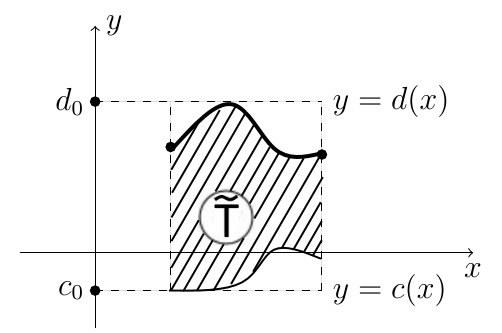
\includegraphics[scale=0.6]{img/631.jpg}
	\end{center}
	Отсюда, используя прямоугольник $\text{П}_0 = [a;b] \times [c_0;d_0]$, в силу аддитивности ОИ и 2И имеем:
	$\displaystyle
    \iint\limits_{\widetilde{T}} f(x,y)dxdy = \iint\limits_{\widetilde{T}} f(x,y)dxdy + \iint\limits_{\text{П}_0 \setminus \widetilde{T}} 0 dxdy = \iint\limits_{\widetilde{T}} f(x,y)dxdy + \iint\limits_{\text{П}_0 \setminus \widetilde{T}} f_0(x,y) dxdy =
    $
    \\
    $
    \displaystyle
    = \iint\limits_{\text{П}_0} f_0(x,y) dxdy = [\eqref{eq:6.3-18}] = \dint\limits_{a}^b dx \dint\limits_{c_0}^{d_0} f_0(x,y) dy =$ \\
	$= \begin{sqcases} \dint\limits_{c_0}^{d_0} f_0(x,y)dy = \dint\limits_{c_0}^{c(x)} f_0(x,y)dx + \dint\limits_{c(x)}^{d(x)} f_0(x,y)dx + \dint\limits_{d(x)}^{d_0} f_0(x,y)dx = \dint\limits_{c(x)}^{d(x)} f_0(x,y)dx \end{sqcases} = $\\
    $= \dint\limits_{a}^{b} dx \dint\limits_{c(x)}^{d(x)}f_0(x, y)dy dy$
	$= \dint\limits_{a}^{b} dx \dint\limits_{c(x)}^{d(x)} f(x,y)dy$.

	Аналогично в случае трапеции \eqref{eq:6.3-21} обосновывается формула \eqref{eq:6.3-22}.
\end{proof}
\newpage

\begin{example}
	Рассмотрим $\displaystyle I = \iint\limits_{x^2 + y^2 \leqslant 2x} f(x,y)dxdy$.

	Для области интегрирования $ T $ следует:
	$x^2 + 2x + y^2 \leqslant 0 \Rightarrow (x-1)^2 + y^2 \leqslant 1$, т.е. $T$ - круг с центром в точке C(1,0) и радиуса $R = 1$.

	\begin{enumerate}
	  \item Если $x \in [0;2]$, то из неравенства $y^2 \leqslant 2x - x^2 \Rightarrow -\sqrt{2x - x^2} \leqslant y \leqslant \sqrt{2x - x^2}$.

		\begin{center}
			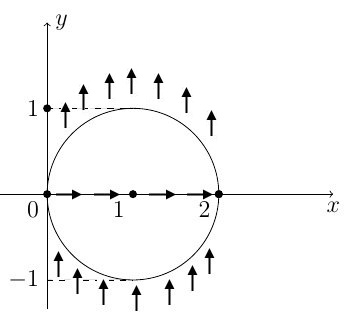
\includegraphics[scale=0.7]{img/632.jpg}
		\end{center}
		В данном случае круг $ T $ можно рассматривать как криволинейную трапецию вдоль оси $ Oy $. Здесь для определения изменения $ x $ следует спроектировать $ T $ на ось $ Ox $ и \important{двигаться по оси $ Ox $}. В результате получаем: $0 \leqslant x \leqslant 2$.

		Для определения линий входа и выхода при движении \important{вдоль оси $ Oy $} имеем:
		\\
		$y = - \sqrt{2x - x^2}$ - линия входа в $ T $, $y =  \sqrt{2x - x^2}$ - линия выхода из $ T $.

		Отсюда в силу \eqref{eq:6.3-20} следует:
		\begin{equation*}
			I = \dint\limits_0^2 dx \dint\limits_{- \sqrt{2x - x^2}}^{\sqrt{2x - x^2}} f(x,y)dy.
		\end{equation*}
	  \item Будем рассматривать наш круг T как криволинейную трапецию вдоль оси $ Ox $, в этом случае проектирование $ T $ на $ Oy $ даёт $ -1 \leqslant y \leqslant 1 $, а при решении уравнения \\
        $(x-1)^2 \leqslant 1-y^2$ получаем:
		$1 - \sqrt{1-y^2} \leqslant x \leqslant 1 + \sqrt{1-y^2}$, \\
        т.е. при движении \important{вдоль оси $ Ox $} имеем:
        \\
		$x = 1 - \sqrt{1 - y^2}$ - линия входа в $ T $, $x = 1 + \sqrt{1 - y^2}$ - линия выхода из $ T $.

		Отсюда в силу \eqref{eq:6.3-22} следует: $I = \dint\limits_{-1}^1 dy \dint\limits_{1 - \sqrt{1 - y^2}}^{1 + \sqrt{1 - y^2}} f(x,y)dx$.
	\end{enumerate}
	Отметим, что на практике для представления 2И через повторные интегралы, в случае более сложных областей интегрирования
	при возможности разбивают используемую область вертикальными и горизонтальными прямыми на соответствующие криволинейные трапеции либо вдоль $ Ox $, либо вдоль $ Oy $.
	Если таких трапеций конечное число, то используют аддитивность 2И и рассматривают пределы интегрирования для каждой трапеции в отдельности.
\end{example}

\subsection{Тройной интеграл}
Рассмотрим $f(x, y, z)$, определённую в $\forall (x, y, z) \in H \subset \R{3}$, где $H$ - измеримое
множество в $\R{3}$, т.е. некоторое кубируемое тело. В данном случае имеем тройной интеграл
\begin{equation}
	\label{eq:6.4-triple-integral}
	I = \iiint\limits_H f(x, y, z)dxdydz.
\end{equation}

\begin{theorem}[о сведении вычисления 3И к 2И]
    Пусть $H$ - цилиндрическое тело вдоль оси $Oz$, т.е:
    \begin{equation}
		\label{eq:6.4-symmetric-body}
		H = \defineset{(x, y, z) \in \R{3}}{(x, y) \in D \subset \R{2}, p \leqslant z \leqslant q},
    \end{equation}
    где $p, q \in \R{}$, а $D$ - квадрируемый компакт в $\R{2}$.

    Если $f \in C(H)$, т.е. непрерывна на $H$, то
    \begin{equation}
		\label{eq:6.4-triple-to-double-integral}
		I \overset{\eqref{eq:6.4-triple-integral}}{=} \iint\limits_D
		\parenthesis{\int\limits_p^q f(x, y, z)dz}dxdy.
    \end{equation}
\end{theorem}

\begin{proof}
    проводится по той же схеме, что и при вычислении 2И по прямоугольнику. Вначале рассматриваем произвольное
    разбиение ${\forall P_0 = \set{z_k}, k = \overline{0, m}}$, отрезка $\interval[{p; q}]$ на части
    ${p = z_0 < z_1 < \ldots < z_{m - 1} < z_m = q}$. В соответствии с этим разбиением, в силу
    непрерывности $f$ на $H$, имеем непрерывную Ф2П:
    \begin{equation}
		\label{eq:6.4-proof-theorem1-e1}
		F(x, y) = \int\limits_p^q f(x, y, z)dz, k = \overline{1, m}.
    \end{equation}
    Далее, проводя произвольное разбиение $\forall \widetilde{P_0}$ квадрируемого компакта
    $D \subset \R{2}$,
    являющегося проекцией $H \subset \R{3}$, на $Oxy$, имеем:
    \begin{center}
        ${T_0 = \set{D_j}, j = \overline{1, l}}$,
        где $\bigcup\limits_{j = 1}^lD_j = D$ и $\mes(D_j \cap D_i) = 0$, ${i \neq j}$.
    \end{center}

    Выбирая произвольным образом множество отмеченных точек:
    \begin{equation*}
		\widetilde{Q_0} = \set{M_j}, \forall M_j = (x_j, y_j) \in D_j, j = \overline{1, l},
    \end{equation*}
    Рассмотрим
    \begin{equation}
		\label{eq:6.4-proof-theorem1-e2}
		I_{kj} = \int\limits_{z_{k - 1}}^{z_k}f(x_j, y_j, z) dz.
    \end{equation}
		По теореме о среднем получаем, что $
        \exists t_{kj} \in \interval[{z_{k - 1}; z_k}] \Rightarrow
		I_{kj} = f(x_j, y_j, t_{kj})(z_k - z_{k-1}) = \linebreak = f(N_{kj})\Delta{z_k}$,
    \begin{equation}
	    \label{eq:6.4-proof-theorem1-e3}
        \text{где }
		\begin{cases}
			N_{kj} = (x_j, y_j, t_{kj}) = (M_j, t_{kj})\\
			\Delta{z_k} = z_k - z_{k - 1}\\
			k = \overline{1, m}, j = \overline{1, l}\\
		\end{cases}
    \end{equation}

    Отсюда при $r_0 = \diam{\widetilde{P_0}} \to 0$ имеем
    \begin{equation}
		\label{eq:6.4-proof-theorem1-e4}
		I_0 = \iint\limits_D F(x, y) dxdy = \lim\limits_{r_0 \to 0}\widetilde{\sigma_0}, \text{ где }
    \end{equation}
    \begin{equation*}
		\begin{split}
			&\widetilde{\sigma_0} = \sigma(F_i(\widetilde{P_0}, \widetilde{Q_0})) =
			\sum\limits_{j = 1}^l F(M_j) \mes D_j = \begin{sqcases}F
				\overset{\eqref{eq:6.4-proof-theorem1-e1}}{=} \dint_p^q fdz = \dint_{z_0=p}^{z_1} + \ldots
				+ \dint_{z_{m - 1}}^{z_m=q} = \sum\limits_{k = 1}^m\dint_{z_{k - 1}}^{z_k}fdz\end{sqcases}=\\
			&=\sum\limits_{j = 1}^l(\sum\limits_{k = 1}^m\dint_{z_{k - 1}}^{z_k} f(M_j, z)dz) \mes D_j
			\overset{\eqref{eq:6.4-proof-theorem1-e2}}{=} \sum\limits_{j = 1}^l\sum\limits_{k = 1}^m
			I_{kj}\mes D_j =
		\end{split}
    \end{equation*}
    \begin{equation}
		\label{eq:6.4-proof-theorem1-e5}
		=\sum\limits_{j = 1}^l\sum\limits_{k = 1}^mf(N_{kj})\Delta{z_k}\mes{D_j}.
    \end{equation}

    Эту сумму \eqref{eq:6.4-proof-theorem1-e5} можно рассматривать как специальную интегральную
    сумму $\sigma_0$ для \eqref{eq:6.4-triple-to-double-integral}, построенную по разбиению
    ${P = (H_{kj})}$ с множеством отмеченных точек
    % $N = (x_j, y_j, t_{kj})$,
    ${Q = \set{N_{kj}}}$, где
    $H_{kj} = D_j \times [{z_{k - 1},  z_k}]$, ${N_{kj} = (x_j, y_j, t_{kj}) \in H_{kj},	  k = \overline{1, m}, j = \overline{1, l}}$. Действительно:
    \begin{equation*}
		\sigma_0 = \sigma_0(f; \set{P, Q}) = \sum\limits_{k = 1}^m\sum\limits_{j = 1}^lf(N_{kj})\mes H_{kj} =
		\begin{sqcases}
			\mes H_{kj} = \text{объём}(D_j \times \interval[{z_{k - 1}; z_k}]) =\\
			=(\text{площадь }D_j)(z_k - z_{k - 1}) = \mes D_j \Delta{z_k}
		\end{sqcases}=
    \end{equation*}
    \begin{equation}
		\label{eq:6.4-proof-theorem1-e6}
		=\sum\limits_{k = 1}^m\sum\limits_{j = 1}^lf(N_{kj})\mes D_j \Delta{z_k}
		\overset{\eqref{eq:6.4-proof-theorem1-e5}}{=} \widetilde{\sigma_0}.
    \end{equation}
    Поэтому, учитывая, что при ${r = \diam P \to 0 \Rightarrow r_0 = \diam \widetilde{P_0} \to 0}$,
    в силу непрерывности $f(x, y, z)$ на компакте $H \subset \R{3}$ имеем:
    \begin{equation*}
		\begin{split}
			&I \overset{\eqref{eq:6.4-proof-theorem1-e1}}{=}
			\lim\limits_{r \to 0}\sigma_0\overset{\eqref{eq:6.4-proof-theorem1-e6}}{=}
			\lim\limits_{r_0 \to 0}\widetilde{\sigma_0 }\overset{\eqref{eq:6.4-proof-theorem1-e4}}{=}
			\iint\limits_D F(x, y)dxdy \overset{\eqref{eq:6.4-symmetric-body}}{=} \iint\limits_D
			\parenthesis{\int\limits_p^q f(x, y, z)dz}dxdy = \\
			&=\iint\limits_D dxdy\int\limits_p^qf(x, y, z)dz
		\end{split}
    \end{equation*}
\end{proof}

\begin{notes}
  \item Если компакт $H \subset \R{3}$ является цилиндроидом вдоль оси $Oz$, т.е:
    \begin{equation*}
		H = \defineset{(x, y, z) \in \R{3}}{p(x, y) \leqslant z \leqslant q(x, y), (x, y) \in D},
    \end{equation*}
    $p(x, y), q(x, y)$ - непрерывные на квадрируемом компакте $D \subset \mathbb{R}^2$, то для $f \in C(H)$:
    \begin{equation}
		\label{eq:6.4-note1}
		I \overset{\eqref{eq:6.4-triple-to-double-integral}}{=} \iint\limits_D \left( \nullFrac\int\limits_{p(x, y)}^{q(x, y)}
		  f(x, y, z) dz \right) dxdy.
    \end{equation}
    $ {
	  \text{
		Обоснование \eqref{eq:6.4-note1} проводится по той же схеме, что и в соответствующем случае для 2И.
	  }
	} $

  \item Если компакт $H \subset \R{3}$ является цилиндроидом \eqref{eq:6.4-note1} вдоль оси $Oz$, где квадрируемый компакт $D \subset \R{2}$ является некоторой
    криволинейной трапецией вдоль оси $Oy$ и, значит,
    \begin{equation*}
		H = \defineset{(x, y, z) \in \R{3}}{p(x, y) \leqslant z \leqslant q(x, y),
		  c(x) \leqslant y \leqslant d(x), a \leqslant x \leqslant b},
    \end{equation*}
    то в случае непрерывности используемых функций получаемое представление для 3И через
    повторные интегралы:
    \begin{equation}
		\label{eq:6.4-note2}
		I \overset{\eqref{eq:6.4-triple-to-double-integral}}{=}
		\int\limits_a^bdx\int\limits_{c(x)}^{d(x)}dy\int_{p(x, y)}^{q(x, y)}f(x, y, z)dz.
    \end{equation}
  \item Формула \eqref{eq:6.4-note2} естественным образом обобщается на случаи соответствующих
    трапеций и цилиндроидов вдоль других координатных осей. В общем
    случае, когда компакт $H \subset \R{3}$ является объединением конечного числа таких цилиндроидов,
    вычисление \eqref{eq:6.4-triple-to-double-integral} в силу аддитивности 3И сводится к вычислению
    интегралов по элементарным цилиндроидам вдоль какой-либо из осей.
\end{notes}

\begin{example}
	Для непрерывной на $\interval[{0; 1}]$ функции $g(z)$ рассмотрим 3И, заданный в виде повторного
	интеграла:
	\begin{equation*}
		I_0 = \int\limits_{-1}^1dx\int\limits_{-\sqrt{1 - x^2}}^{\sqrt{1 - x^2}}\int\limits_{x^2+y^2}^1 g(z)dz.
	\end{equation*}
	В данном случае имеем:
	\begin{equation*}
		I_0 \overset{\eqref{eq:6.4-triple-to-double-integral}}{=}\iiint\limits_Hg(z)dxdydz,
	\end{equation*}
	где $H$ - компакт в $\R{3}$, ограниченный в пространстве параболоидом ${z = x^2 + y^2}$ и
	плоскостью $z = 1$, проекцией которого на $Oxy$ является круг $D: x^2 + y^2 \leqslant 1$:
\begin{center}
	  [IMAGE NOT FOUND]
		% \includegraphics[scale=0.7]{img/635.jpg}
\end{center}
	Рассматривая $H$ как соответствующий  элементарный цилиндроид вдоль $Oy$, имеем:
	\begin{equation*}
		H = \defineset{(x, y, z) \in \R{3}}{\sqrt{z - x^2} \leqslant y \leqslant \sqrt{z - x^2},
		  -\sqrt{z} \leqslant x \leqslant \sqrt{z}, 0 \leqslant z \leqslant 1}
	\end{equation*}
	Переходя в таком виде снова к повторному интегралу, получаем:
	\begin{equation*}
		\begin{split}
			&I_0 = \int\limits_0^1dz\int\limits_{-\sqrt{z}}^{\sqrt{z}}dx\int\limits_{-\sqrt{z - x^2}}^{\sqrt{z - x^2}}g(z)dy =
			\int\limits_0^1dz\int\limits_{-\sqrt{z}}^{\sqrt{z}} \begin{sqcases} yg(z) \end{sqcases}_{y = -\sqrt{z - x^2}}^{y = \sqrt{z - x^2}} dx =
			2\int\limits_0^1dz\int\limits_{-\sqrt{z}}^{\sqrt{z}}g(z)\sqrt{z - x^2}dx =\\
			&=\begin{sqcases}\dint\sqrt{a^2 - x^2}dx = \frac{x}{2}\sqrt{a^2 - x^2} + \frac{a^2}{2}\arcsin{\frac{x}{a}} + c\end{sqcases} =
			4\dint\limits_0^1g(z)
			\begin{sqcases}\frac{x}{2}\sqrt{z - x^2} + \frac{z}{2}\arcsin{\frac{x}{\sqrt{z}}}\end{sqcases}_{x = 0}^{x = \sqrt{z}}dz =\\
			&=4\int\limits_0^1g(z)\frac{\pi z}{4}dz = \pi\int\limits_0^1zg(z)dz.
		\end{split}
	\end{equation*}
	Изменив порядок интегрирования мы свели вычисление тройного интеграла к вычислению
	соответствующего однократного интеграла.
\end{example}

\subsection{Замена переменных в $n$-кратном интеграле}
Рассмотрим множества $D \subset \R{n}$ и $G \subset \R{n}$. Множество $D$ будем рассматривать в системе координат $O_{x_1,\ldots x_n}$,
а множество $G$ - в системе координат $O_{t_1,\ldots t_n}$.

Пусть имеется отображение
\begin{equation}
	\label{eq:lecture6-34}
	f : G \to D,
\end{equation}
при котором $\forall t = (t_1, \ldots t_n) \in G$ ставится в соответствие
единственное ${f(t) = (f_1(t), \ldots f_n(t)) \in D}$. Отображение \eqref{eq:lecture6-34}
будет взаимно-однозначным, если оно инъективно, т.е. различным точкам из $G$
будут соответствовать различные точечные образы в $D$.

В случае взаимной одозначности \eqref{eq:lecture6-34} существует единственное
обратное отображение
\begin{equation}
	\label{eq:lecture6-35}
	g : D \to G,
\end{equation}
при котором $\forall x \in D \exists ! t = g(x) \in G \suchthat f(t) = x$.

Если во взаимооднозначных соотношениях \eqref{eq:lecture6-34}, \eqref{eq:lecture6-35}
используется непрерывно дифференцируемая функция, то говорят, что множества $D$
и $G$ \important{диффеоморфны}, а отображения \eqref{eq:lecture6-34},
\eqref{eq:lecture6-35} - диффеоморфизмы.

Для диффеоморфизма \eqref{eq:lecture6-34} его Якобиан - это определитель
\begin{equation}
	\label{eq:lecture6-36}
	J(t) = \det\dfrac{\partial F}{\partial t} =
	\begin{vmatrix}
		\frac{\partial F_1}{\partial t_1} & \ldots & \frac{\partial F_1}{\partial t_n}\\
		\vdots & \ddots & \vdots\\
		\frac{\partial F_n}{\partial t_1} & \ldots & \frac{\partial F_n}{\partial t_n}\\
	\end{vmatrix}.
\end{equation}
Якобиан обратного диффеоморфного отображения \eqref{eq:lecture6-35} будем обозначать
\begin{equation}
	\label{eq:lecture6-37}
	\mathcal{J}(t) = \det\dfrac{\partial g}{\partial x} =
	\begin{vmatrix}
		\frac{\partial g_1}{\partial x_1} & \ldots & \frac{\partial g_1}{\partial x_n}\\
		\vdots & \ddots & \vdots\\
		\frac{\partial g_n}{\partial x_1} & \ldots & \frac{\partial g_n}{\partial x_n}\\
	\end{vmatrix}.
\end{equation}

Используя свойства определителя можно показать, что \eqref{eq:lecture6-36} и
\eqref{eq:lecture6-37} удовлетворяют условию $J(t) \mathcal{J}(t) = 1$, откуда, в
 частности, следует, что при диффеоморфизме \eqref{eq:lecture6-34} и \eqref{eq:lecture6-35} якобианы \eqref{eq:lecture6-36} и
\eqref{eq:lecture6-37} - ненулевые определители.

Можно показать, что диффеоморфизме \eqref{eq:lecture6-34} для меры $\mes  G$ образа и меры прообраза $\mes D$ имеем:
\begin{equation}
	\label{eq:measure-statement}
	\mes D = \int_G \abs{f(t)}dt = \underset{G}{\int \ldots \int}\abs{J(t_1, \ldots t_n)}dt_1 \ldots dt_n
\end{equation}
Обоснование \eqref{eq:measure-statement} для случая $n = 2$ и $n = 3$ будет сделано позже.

\begin{theorem}[о замене переменных в $ n $-кратном интеграле]$  $

    Если для диффеоморфизма \eqref{eq:lecture6-34} и для функции $ h $ существует непрерывная композиция ${ ( h \circ f)(t) =h(f(t)) = h(f_1(t), \ldots, f_n(t))}, t \in G \subset \RN$,
    то тогда:
    \begin{equation}
        \dint\limits_D h(x) dx =
        \begin{sqcases}
            x = f(t) \text{ - непрерывно дифференцируема в } D, \\
            dx \overset{\eqref{eq:lecture6-34}}{=} \abs{J(t)} \; dt
        \end{sqcases}
        =
        \dint\limits_G h(f(t)) \; \abs{J(t)} \; dt.
    \end{equation}
\end{theorem}

\begin{proof}
	Для доказательства воспользуемся \eqref{eq:measure-statement} в предположении,
	что $D$, а значит, и $G$ в \eqref{eq:lecture6-34} являются измеримыми компактами в $\R{n}$.

	Возьмём $\forall P = \set{D_k}$ - произвольное разбиение измеримого компакта
	$D \subset \R{n}$ на измеримые компакты $D_k, k = \overline{1, m}$.
	Имеем:
    ${\bigcup\limits_{k = 1}^mD_k = D}$ и ${\mes(D_i \cap D_j) = 0, \forall i \neq j}$.

	При диффеоморфизме \eqref{eq:lecture6-34}, \eqref{eq:lecture6-35} рассматриваемое
	разбиение $P$ множества $D$ порождает соответствующие разбиения S измеримого
	компакта $G \subset \R{2}$ на измеримые компактные части $G_k = g(D_k)$,
	является образом обратного \eqref{eq:lecture6-34} диффеоморфизма
	\eqref{eq:lecture6-35}, причём 	${\bigcup\limits_{k = 1}^mG_k = G}$ и ${\mes(G_i \cap G_j) = 0, \forall i \neq j}$. Используя теорему о среднем для
	$n$-кратного интеграла, в силу \eqref{eq:measure-statement} имеем:
	\begin{equation}
		\label{eq:diffeomorph-measure}
		\Delta D_k = \mes D_k \overset{\eqref{eq:measure-statement}}{=} \intl_{G_k} \abs{J(t)}dt =
		\begin{sqcases}\exists N_k \in S_k\end{sqcases} =
		\abs{J(N_k)}\Delta{G_k}
	\end{equation}
	где
	\begin{equation*}
		\Delta G_k = \mes G_k = \intl_{G_k}dt
	\end{equation*}

	Полученное таким образом для разбиения $S$ компакта $G \subset \R{n}$ множество отмеченных точек
	$T = \set{N_k}, \forall N_k \in G_k, k = \overline{1, n},$ даёт для разбиения $P$ компакта
	$D \subset \R{n}$ соответствующее множество $Q = \set{M_k}$ отмеченных точек $M_k \overset{\eqref{eq:lecture6-34}}{=} f(N_k) \in D_k, k = \overline{1, m}$.

	Отсюда для интегральной суммы
	\begin{equation}
		\label{eq:diffeomorph-integral-summ}
		\sigma = \sigma(h; \set{P; Q}) = \sum_{k = 1}^m h(N_k)\Delta D_k
	\end{equation}
	получаем:
	\begin{equation}
		\label{eq:diffeomorph-integral-sum-result}
		\sigma \overset{\eqref{eq:diffeomorph-measure}}{=} \sum_{k = 1}^mh(f(N_k)) \abs{J(N_k)} \Delta G_k,
	\end{equation}
	то есть $\sigma = \sigma(H, \set{S; T})$, где $H(t) = \abs{J(t)}h(f(t))$.

	При этом для \eqref{eq:lecture6-34}, \eqref{eq:lecture6-35} следует:
	\begin{equation*}
		r = \diam P \to 0 \Leftrightarrow d = \diam S \to 0.
	\end{equation*}
    
	Поэтому в силу
	непрерывности используемой ФНП для предела полученной специальной
	интегральной суммы имеем:
	\begin{equation*}
		\int_D h(x)dx \overset{\eqref{eq:diffeomorph-integral-summ}}{=}
		\lim\limits_{r \to 0}\sigma(h; \set{P; Q}) = \lim\limits_{d \to 0}\sigma(H; \set{S; T}) =
		\int_G H(t)dt = \int_G \abs{J(t)}h(f(t))dt.
	\end{equation*}
\end{proof}

%\textbf{  Замечания о замене переменных в 2И и 3И. }
\begin{notes}
  \item В случае $n = 2$ для полярной замены переменных
	\begin{equation*}
		\begin{cases}
			x = r \cos \phi\\
			y = r \sin \phi\\
		\end{cases}
	\end{equation*}
	якобиан равен
	\begin{equation*}
		I = \dfrac{\partial(x, y)}{\partial(r, \varphi)} =
		\begin{vmatrix}
			x'_r & x'_{\varphi}\\
			y'_r & y'_{\varphi}\\
		\end{vmatrix} =
		\begin{vmatrix}
			\cos \varphi & -r \sin \varphi\\
			\sin \varphi & r \cos \varphi\\
		\end{vmatrix} = r \geqslant 0.
	\end{equation*}
	Поэтому, если для использованных квадрируемых компактов $D$ и $G$ в $\R{2} \Rightarrow r > 0$,
	то для непрерывной функции двух переменных $h = h(x, y), (x, y) \in D(h), (r, \varphi) \in E(h)$,
	в силу доказанной теоремы, получаем формулу полярной замены:
	\begin{equation}
		\label{eq:2d-integral-vars}        
        \iintl_D h(x, y)dxdy =
        \begin{sqcases}
        x = r \cos \varphi\\
        y = r \sin \varphi\\
        I = r > 0
        \end{sqcases} =
		   \iintl_G r h(r\cos \varphi, r \sin \varphi) dr d\varphi.
	\end{equation}
  \item Аналогично, в случае $n = 3$ рассматриваем цилиндрическую замену
	\begin{equation*}
		\begin{cases}
			x = r \cos \varphi,\\
			y = r \sin \varphi,\\
			z = z,
		\end{cases}
	\end{equation*}
	соответствующую в $\R{3}$ полярной замене. Для якобиана $I(r, \varphi, z)$ получаем:
	\begin{equation*}
		I(r, \varphi, z) =
		\begin{vmatrix}
			x'_r & x'_{\varphi} & 0\\
			y'_r & y'_{\varphi} & 0\\
			0 & 0 & 1
		\end{vmatrix} =
		\begin{vmatrix}
			x'_r & x'_{\varphi}\\
			y'_r & y'_{\varphi}\\
		\end{vmatrix} = r > 0.
	\end{equation*}
	В результате для непрерывной функции $h = h(x, y, z)$, в случае, когда $r > 0$, имеем:
	\begin{equation}    
		\label{eq:2d-cylindrir-integral-vars}        
        \iiint\limits_D h(x, y, z) dxdydz =
        \begin{sqcases}
        x = r \cos \varphi,\\
        y = r \sin \varphi,\\
        z = z, \\
        I = r \geqslant 0
        \end{sqcases} =        
		\iiint\limits_G r h(r \cos \varphi, r \sin \varphi, z)dr d\varphi dz.
	\end{equation}
  \item Рассмотрим в пространстве $(n = 3)$ сферическую замену:
	\begin{equation*}
		\begin{cases}
			x = r \cos \varphi \cos \psi\\
			y = r \sin \varphi \cos \psi\\
			z = r \sin \psi,\\
		\end{cases}
		r \geqslant 0, 0 \leqslant \varphi \leqslant 2 \pi, -\dfrac{\pi}{2} \leqslant \psi \leqslant \dfrac{\pi}{2}.
	\end{equation*}
	В данном случае для якобиана со сферической заменой следует:
	\begin{equation*}
		I =
		dt \dfrac{\partial(x, y, z)}{\partial(r, \varphi, \psi)} =
		\begin{vmatrix}
			x'_r & x'_{\varphi} & x'_{\psi}\\
			y'_r & y'_{\varphi} & y'_{\psi}\\
			z'_r & z'_{\varphi} & z'_{\psi}\\
		\end{vmatrix} = \ldots = r^2\cos\psi \geqslant 0.
	\end{equation*}
	Поэтому, если для используемых кубируемых компактов $D$ и $G$ в $\R{3}$ имеем $r > 0$ и
	${\varphi \ne \pm \dfrac{\pi}{2}}$, то якобиан $I(r, \varphi, \psi) > 0$, и в этом случае имеем
	следующую формулу сферической замены для непрерывной Ф3П $h(x, y, z)$:
	\begin{equation}
		\label{eq:3d-sphere}
        \begin{split}
                \iiint_D h(x, y, z) \; dxdydz =
                \begin{sqcases}
                x = r \cos \varphi \cos \psi\\
                y = r \sin \varphi \cos \psi\\
                z = r \sin \psi,\\
                I = r^2 \cos \psi > 0.
                \end{sqcases} = \\
                =\iiint_G r^2 h(r \cos \varphi \cos \psi, r \sin \varphi \cos \psi, r \sin \psi) \cos \psi dr d\varphi d\psi.
        \end{split}
	\end{equation}
\end{notes}
\begin{statement}{Упражнения} \begin{enumerate}
    \item Показать, что якобиан $J(r, \phi)$ обобщённой полярной замены
	\begin{equation*}
		\begin{cases}
			&x = ar \cos^{\alpha}\phi,\\
			&y = br \sin^{\alpha}\phi,\\
			&a, b, \alpha \in \R{}.\\
		\end{cases}
	\end{equation*}
	равен $J(r, \phi) = \alpha abr \cos^{\alpha - 1}\phi\sin^{\alpha - 1}\phi$. Исходя из этого,
	записать формулу обобщённой полярной замены в 2И.

	\item Показать, что Якобиан $J(r, \phi, \psi)$ обобщённой сферической замены
	\begin{equation*}
		\begin{cases}
			&x = ar \cos^{\alpha}\phi\cos^{\beta}\psi,\\
			&y = br \sin^{\alpha}\phi\cos^{\beta}\psi,\\
			&z = cr \sin^{\beta}\psi,\\
			&a, b, c, \alpha, \beta \in \R{}.\\
		\end{cases}
	\end{equation*}
	равен $J(r, \phi, \psi) = \alpha \beta abcr^2 \cos^{\alpha - 1}\phi\sin^{\alpha - 1}\phi
	\cos^{2\beta - 1}\psi\sin^{\beta - 1}\beta$. Исходя из этого, записать соответствующую
	формулу замены переменных в обобщённой полярной системе координат.
\end{enumerate} \end{statement}

\begin{note}
	На практике формулы \eqref{eq:diffeomorph-integral-sum-result}, \eqref{eq:2d-integral-vars} и \eqref{eq:2d-cylindrir-integral-vars} часто можно
	использовать и в случае, когда используемые якобианы для рассматриваемых измеримых компактов
	$D$ и $G$ обращаются в ноль в отдельных точках.
\end{note}

\begin{examples}
  \item Пусть $I = \diint\limits_{x^2 + y^2 \leqslant 2x + 2y}(x + y)dxdy$. 
  
	\begin{equation*}
		(x^2 - 2x) + (y^2 - 2x) \leqslant 0 \Leftrightarrow
		(x - 1)^2 + (y - 1)^2 \leqslant 2 \text{ - круг с центром в $(1, 1)$
		и радиусом $R = \sqrt{2}$}.
	\end{equation*}
	Вход: $r = 0$, выход: $x^2 + y^2 = 2(x + y) \Leftrightarrow$
	\begin{equation*}
		\Leftrightarrow r^2 = 2r(\cos \phi + \sin \phi) \Leftrightarrow
		r = 2(\cos \phi + \sin \phi), \text{ т.е. } 0 \leqslant r \leqslant
		2(\cos \phi + \sin \phi), -\frac{\pi}{4} \leqslant \phi \leqslant \frac{3 \pi}{4}.
	\end{equation*}
	Отсюда $I = \iint\limits_G r^2 (\cos \phi + \sin \phi) dr d \phi =$ 
	\begin{equation*}
		\begin{split}
			&=\int\limits_{-\frac{\pi}{4}}^{\frac{3\pi}{4}}\sqcase{\dfrac{r^3(\cos \phi + \sin \phi)}{3}}_
			{r = 0}^{r = 2(\cos \phi + \sin \phi)}d\phi =
			\dfrac{8}{3}\int\limits_{-\frac{\pi}{4}}^{\frac{3\pi}{4}}
			(\cos \phi + \sin \phi)^3d\phi
			=\\
			&=\dfrac{8}{3}\int\limits_{-\frac{\pi}{4}}^{\frac{3\pi}{4}}
			(\cos \phi + \sin \phi)^2d(\sin \phi - \cos \phi)=
			\dfrac{8}{3}\int\limits_{-\frac{\pi}{4}}^{\frac{3\pi}{4}}
			(2 -( \sin \phi - \cos \phi)^2)\; d(\sin \phi - \cos \phi)=\\
			&=\dfrac{8}{3}\sqcase{2(\sin \phi - \cos \phi) -
			  \dfrac{(\sin \phi - \cos \phi)^3}{3}}_{-\frac{\pi}{4}}^{\frac{3\pi}{4}} = \dfrac{64\sqrt{2}}{9}.
		\end{split}
	\end{equation*}
  \item Пусть $I = \diint\limits_Dxydxdy$, где
	\begin{equation*}
		D:
		\begin{cases}
			&xy = 1,\\
			&xy = 4,\\
			&y = \frac{x}{4},\\
			&y = 4x,\\
			&x \geqslant 0,\\
			&y \geqslant 0,\\
		\end{cases}
	\end{equation*}
	Воспользуемся общей заменой:
	\begin{equation*}
    u = (xy) \suchthat_1^4, 
		v = \left.\parenthesis{\dfrac{y}{x}}\right|_{1/4}^4, \mathcal{J} = \det\dfrac{\partial(u, v)}
		{\partial(x, y)} =
		\begin{vmatrix}
			u'_x & u'_y\\
			v'_x & v'_y\\
		\end{vmatrix} =
		\begin{vmatrix}
			y & x\\
			-\frac{y}{x^2} & \frac{1}{x}\\
		\end{vmatrix} = 2\dfrac{y}{x} = 2v, J = \dfrac{1}{\mathcal{J}} = \dfrac{1}{2v}.
	\end{equation*}
	В данном случае для подынтегральной функции $ h(x, y) = xy = u $ получаем:    
	\begin{equation*}
		\begin{split}
			& I = \iint\limits_Gu\abs{\dfrac{1}{2v}}dudv =
			\int\limits_1^4udu \cdot \int\limits_{1/4}^4\dfrac{dv}{2v} =\\
			&=\parenthesis{\sqcase{\dfrac{4^2}{2}}_1^4}\cdot
			\parenthesis{\sqcase{\dfrac{1}{2}\ln v}_{1/4}^4} =
			\dfrac{15}{2} \cdot \dfrac{1}{2} \parenthesis{\ln 4 - \ln \dfrac{1}{4}} = 15 \ln 2.
		\end{split}
	\end{equation*}
\end{examples}